% THIS TEMPLATE_article_for_IJET_jrnl.tex is based on
%% bare_jrnl.tex
%% V1.3
%% 2007/01/11
%% by Michael Shell
%% see http://www.michaelshell.org/
%% for current contact information.
%%
%% This is a skeleton file demonstrating the use of IEEEtran.cls
%% (requires IEEEtran.cls version 1.7 or later) with an IEEE journal paper.
%%
%% Support sites:
%% http://www.michaelshell.org/tex/ieeetran/
%% http://www.ctan.org/tex-archive/macros/latex/contrib/IEEEtran/
%% and
%% http://www.ieee.org/



% *** Authors should verify (and, if needed, correct) their LaTeX system  ***
% *** with the testflow diagnostic prior to trusting their LaTeX platform ***
% *** with production work. IEEE's font choices can trigger bugs that do  ***
% *** not appear when using other class files.                            ***
% The testflow support page is at:
% http://www.michaelshell.org/tex/testflow/


%%*************************************************************************
%% Legal Notice:
%% This code is offered as-is without any warranty either expressed or
%% implied; without even the implied warranty of MERCHANTABILITY or
%% FITNESS FOR A PARTICULAR PURPOSE!
%% User assumes all risk.
%% In no event shall IEEE or any contributor to this code be liable for
%% any damages or losses, including, but not limited to, incidental,
%% consequential, or any other damages, resulting from the use or misuse
%% of any information contained here.
%%
%% All comments are the opinions of their respective authors and are not
%% necessarily endorsed by the IEEE.
%%
%% This work is distributed under the LaTeX Project Public License (LPPL)
%% ( http://www.latex-project.org/ ) version 1.3, and may be freely used,
%% distributed and modified. A copy of the LPPL, version 1.3, is included
%% in the base LaTeX documentation of all distributions of LaTeX released
%% 2003/12/01 or later.
%% Retain all contribution notices and credits.
%% ** Modified files should be clearly indicated as such, including  **
%% ** renaming them and changing author support contact information. **
%%
%% File list of work: IEEEtran.cls, IEEEtran_HOWTO.pdf, bare_adv.tex,
%%                    bare_conf.tex, bare_jrnl.tex, bare_jrnl_compsoc.tex
%%*************************************************************************

% Note that the a4paper option is mainly intended so that authors in
% countries using A4 can easily print to A4 and see how their papers will
% look in print - the typesetting of the document will not typically be
% affected with changes in paper size (but the bottom and side margins will).
% Use the testflow package mentioned above to verify correct handling of
% both paper sizes by the user's LaTeX system.
%
% Also note that the "draftcls" or "draftclsnofoot", not "draft", option
% should be used if it is desired that the figures are to be displayed in
% draft mode.
%

%
% If IEEEtran.cls has not been installed into the LaTeX system files,
% manually specify the path to it like:
% \documentclass[journal]{../sty/IEEEtran}


% Some very useful LaTeX packages include:
% (uncomment the ones you want to load)


% *** CITATION PACKAGES ***
%
%\usepackage{cite}
% cite.sty was written by Donald Arseneau
% V1.6 and later of IEEEtran pre-defines the format of the cite.sty package
% \cite{} output to follow that of IEEE. Loading the cite package will
% result in citation numbers being automatically sorted and properly
% \'compressed/ranged". e.g., [1], [9], [2], [7], [5], [6] without using
% cite.sty will become [1], [2], [5]--[7], [9] using cite.sty. cite.sty's
% \cite will automatically add leading space, if needed. Use cite.sty's
% noadjust option (cite.sty V3.8 and later) if you want to turn this off.
% cite.sty is already installed on most LaTeX systems. Be sure and use
% version 4.0 (2003-05-27) and later if using hyperref.sty. cite.sty does
% not currently provide for hyperlinked citations.
% The latest version can be obtained at:
% http://www.ctan.org/tex-archive/macros/latex/contrib/cite/
% The documentation is contained in the cite.sty file itself.


% *** GRAPHICS RELATED PACKAGES ***
%
%\ifCLASSINFOpdf
  % \usepackage[pdftex]{graphicx}
  % declare the path(s) where your graphic files are
  % \graphicspath{{../pdf/}{../jpeg/}}
  % and their extensions so you won't have to specify these with
  % every instance of \includegraphics
  % \DeclareGraphicsExtensions{.pdf,.jpeg,.png}
%\else
  % or other class option (dvipsone, dvipdf, if not using dvips). graphicx
  % will default to the driver specified in the system graphics.cfg if no
  % driver is specified.
  % \usepackage[dvips]{graphicx}
  % declare the path(s) where your graphic files are
  % \graphicspath{{../eps/}}
  % and their extensions so you won't have to specify these with
  % every instance of \includegraphics
  % \DeclareGraphicsExtensions{.eps}
%\fi
% graphicx was written by David Carlisle and Sebastian Rahtz. It is
% required if you want graphics, photos, etc. graphicx.sty is already
% installed on most LaTeX systems. The latest version and documentation can
% be obtained at:
% http://www.ctan.org/tex-archive/macros/latex/required/graphics/
% Another good source of documentation is "Using Imported Graphics in
% LaTeX2e" by Keith Reckdahl which can be found as epslatex.ps or
% epslatex.pdf at: http://www.ctan.org/tex-archive/info/
%
% latex, and pdflatex in dvi mode, support graphics in encapsulated
% postscript (.eps) format. pdflatex in pdf mode supports graphics
% in .pdf, .jpeg, .png and .mps (metapost) formats. Users should ensure
% that all non-photo figures use a vector format (.eps, .pdf, .mps) and
% not a bitmapped formats (.jpeg, .png). IEEE frowns on bitmapped formats
% which can result in "jaggedy"/blurry rendering of lines and letters as
% well as large increases in file sizes.
%
% You can find documentation about the pdfTeX application at:
% http://www.tug.org/applications/pdftex


% *** MATH PACKAGES ***
%
%\usepackage[cmex10]{amsmath}
% A popular package from the American Mathematical Society that provides
% many useful and powerful commands for dealing with mathematics. If using
% it, be sure to load this package with the cmex10 option to ensure that
% only type 1 fonts will utilized at all point sizes. Without this option,
% it is possible that some math symbols, particularly those within
% footnotes, will be rendered in bitmap form which will result in a
% document that can not be IEEE Xplore compliant!
%
% Also, note that the amsmath package sets \interdisplaylinepenalty to 10000
% thus preventing page breaks from occurring within multiline equations. Use:
%\interdisplaylinepenalty=2500
% after loading amsmath to restore such page breaks as IEEEtran.cls normally
% does. amsmath.sty is already installed on most LaTeX systems. The latest
% version and documentation can be obtained at:
% http://www.ctan.org/tex-archive/macros/latex/required/amslatex/math/


% *** SPECIALIZED LIST PACKAGES ***
%
%\usepackage{algorithmic}
% algorithmic.sty was written by Peter Williams and Rogerio Brito.
% This package provides an algorithmic environment fo describing algorithms.
% You can use the algorithmic environment in-text or within a figure
% environment to provide for a floating algorithm. Do NOT use the algorithm
% floating environment provided by algorithm.sty (by the same authors) or
% algorithm2e.sty (by Christophe Fiorio) as IEEE does not use dedicated
% algorithm float types and packages that provide these will not provide
% correct IEEE style captions. The latest version and documentation of
% algorithmic.sty can be obtained at:
% http://www.ctan.org/tex-archive/macros/latex/contrib/algorithms/
% There is also a support site at:
% http://algorithms.berlios.de/index.html
% Also of interest may be the (relatively newer and more customizable)
% algorithmicx.sty package by Szasz Janos:
% http://www.ctan.org/tex-archive/macros/latex/contrib/algorithmicx/


% *** ALIGNMENT PACKAGES ***
%
%\usepackage{array}
% Frank Mittelbach's and David Carlisle's array.sty patches and improves
% the standard LaTeX2e array and tabular environments to provide better
% appearance and additional user controls. As the default LaTeX2e table
% generation code is lacking to the point of almost being broken with
% respect to the quality of the end results, all users are strongly
% advised to use an enhanced (at the very least that provided by array.sty)
% set of table tools. array.sty is already installed on most systems. The
% latest version and documentation can be obtained at:
% http://www.ctan.org/tex-archive/macros/latex/required/tools/


%\usepackage{mdwmath}
%\usepackage{mdwtab}
% Also highly recommended is Mark Wooding's extremely powerful MDW tools,
% especially mdwmath.sty and mdwtab.sty which are used to format equations
% and tables, respectively. The MDWtools set is already installed on most
% LaTeX systems. The lastest version and documentation is available at:
% http://www.ctan.org/tex-archive/macros/latex/contrib/mdwtools/


% IEEEtran contains the IEEEeqnarray family of commands that can be used to
% generate multiline equations as well as matrices, tables, etc., of high
% quality.


%\usepackage{eqparbox}
% Also of notable interest is Scott Pakin's eqparbox package for creating
% (automatically sized) equal width boxes - aka \'natural width parboxes".
% Available at:
% http://www.ctan.org/tex-archive/macros/latex/contrib/eqparbox/

% *** SUBFIGURE PACKAGES ***
%\usepackage[tight,footnotesize]{subfigure}
% subfigure.sty was written by Steven Douglas Cochran. This package makes it
% easy to put subfigures in your figures. e.g., "Figure 1a and 1b". For IEEE
% work, it is a good idea to load it with the tight package option to reduce
% the amount of white space around the subfigures. subfigure.sty is already
% installed on most LaTeX systems. The latest version and documentation can
% be obtained at:
% http://www.ctan.org/tex-archive/obsolete/macros/latex/contrib/subfigure/
% subfigure.sty has been superceeded by subfig.sty.


%\usepackage[caption=false]{caption}
%\usepackage[font=footnotesize]{subfig}
% subfig.sty, also written by Steven Douglas Cochran, is the modern
% replacement for subfigure.sty. However, subfig.sty requires and
% automatically loads Axel Sommerfeldt's caption.sty which will override
% IEEEtran.cls handling of captions and this will result in nonIEEE style
% figure/table captions. To prevent this problem, be sure and preload
% caption.sty with its \'caption=false" package option. This is will preserve
% IEEEtran.cls handing of captions. Version 1.3 (2005/06/28) and later
% (recommended due to many improvements over 1.2) of subfig.sty supports
% the caption=false option directly:
%\usepackage[caption=false,font=footnotesize]{subfig}
%
% The latest version and documentation can be obtained at:
% http://www.ctan.org/tex-archive/macros/latex/contrib/subfig/
% The latest version and documentation of caption.sty can be obtained at:
% http://www.ctan.org/tex-archive/macros/latex/contrib/caption/


% *** FLOAT PACKAGES ***
%
%\usepackage{fixltx2e}
% fixltx2e, the successor to the earlier fix2col.sty, was written by
% Frank Mittelbach and David Carlisle. This package corrects a few problems
% in the LaTeX2e kernel, the most notable of which is that in current
% LaTeX2e releases, the ordering of single and double column floats is not
% guaranteed to be preserved. Thus, an unpatched LaTeX2e can allow a
% single column figure to be placed prior to an earlier double column
% figure. The latest version and documentation can be found at:
% http://www.ctan.org/tex-archive/macros/latex/base/


%\usepackage{stfloats}
% stfloats.sty was written by Sigitas Tolusis. This package gives LaTeX2e
% the ability to do double column floats at the bottom of the page as well
% as the top. (e.g., "\begin{figure*}[!b]" is not normally possible in
% LaTeX2e). It also provides a command:
%\fnbelowfloat
% to enable the placement of footnotes below bottom floats (the standard
% LaTeX2e kernel puts them above bottom floats). This is an invasive package
% which rewrites many portions of the LaTeX2e float routines. It may not work
% with other packages that modify the LaTeX2e float routines. The latest
% version and documentation can be obtained at:
% http://www.ctan.org/tex-archive/macros/latex/contrib/sttools/
% Documentation is contained in the stfloats.sty comments as well as in the
% presfull.pdf file. Do not use the stfloats baselinefloat ability as IEEE
% does not allow \baselineskip to stretch. Authors submitting work to the
% IEEE should note that IEEE rarely uses double column equations and
% that authors should try to avoid such use. Do not be tempted to use the
% cuted.sty or midfloat.sty packages (also by Sigitas Tolusis) as IEEE does
% not format its papers in such ways.


%\ifCLASSOPTIONcaptionsoff
%  \usepackage[nomarkers]{endfloat}
% \let\MYoriglatexcaption\caption
% \renewcommand{\caption}[2][\relax]{\MYoriglatexcaption[#2]{#2}}
%\fi
% endfloat.sty was written by James Darrell McCauley and Jeff Goldberg.
% This package may be useful when used in conjunction with IEEEtran.cls'
% captionsoff option. Some IEEE journals/societies require that submissions
% have lists of figures/tables at the end of the paper and that
% figures/tables without any captions are placed on a page by themselves at
% the end of the document. If needed, the draftcls IEEEtran class option or
% \CLASSINPUTbaselinestretch interface can be used to increase the line
% spacing as well. Be sure and use the nomarkers option of endfloat to
% prevent endfloat from "marking" where the figures would have been placed
% in the text. The two hack lines of code above are a slight modification of
% that suggested by in the endfloat docs (section 8.3.1) to ensure that
% the full captions always appear in the list of figures/tables - even if
% the user used the short optional argument of \caption[]{}.
% IEEE papers do not typically make use of \caption[]'s optional argument,
% so this should not be an issue. A similar trick can be used to disable
% captions of packages such as subfig.sty that lack options to turn off
% the subcaptions:
% For subfig.sty:
% \let\MYorigsubfloat\subfloat
% \renewcommand{\subfloat}[2][\relax]{\MYorigsubfloat[]{#2}}
% For subfigure.sty:
% \let\MYorigsubfigure\subfigure
% \renewcommand{\subfigure}[2][\relax]{\MYorigsubfigure[]{#2}}
% However, the above trick will not work if both optional arguments of
% the \subfloat/subfig command are used. Furthermore, there needs to be a
% description of each subfigure *somewhere* and endfloat does not add
% subfigure captions to its list of figures. Thus, the best approach is to
% avoid the use of subfigure captions (many IEEE journals avoid them anyway)
% and instead reference/explain all the subfigures within the main caption.
% The latest version of endfloat.sty and its documentation can obtained at:
% http://www.ctan.org/tex-archive/macros/latex/contrib/endfloat/
%
% The IEEEtran \ifCLASSOPTIONcaptionsoff conditional can also be used
% later in the document, say, to conditionally put the References on a
% page by themselves.


% *** PDF, URL AND HYPERLINK PACKAGES ***
%
%\usepackage{url}
% url.sty was written by Donald Arseneau. It provides better support for
% handling and breaking URLs. url.sty is already installed on most LaTeX
% systems. The latest version can be obtained at:
% http://www.ctan.org/tex-archive/macros/latex/contrib/misc/
% Read the url.sty source comments for usage information. Basically,
% \url{my_url_here}.


% *** Do not adjust lengths that control margins, column widths, etc. ***
% *** Do not use packages that alter fonts (such as pslatex).         ***
% There should be no need to do such things with IEEEtran.cls V1.6 and later.
% (Unless specifically asked to do so by the journal or conference you plan
% to submit to, of course. )

%%%%%%%%%%%%%%%%%%%%%%%%%%%%%%%%%%%%%%%%%%%%%%%%%%%%%%%%%%%%%%%%%%%%%%%%%%%%%%%%%%%%%%%%%%%%%%%%%%%%%%%%%%%%%%%%%%%%%%%%%%%%
%%%%%%%%%%%%%%%%%%%%%%%%%%%%%%%%%%%%%%%%%%%%%%%%%%%%%%%%%%%%%%%%%%%%%%%%%%%%%%%%%%%%%%%%%%%%%%%%%%%%%%%%%%%%%%%%%%%%%%%%%%%%
%%%%%%%%%%%%%%%%%%%%%%%%%%%%%%%%%%%%%%%%%%%%%%%%%%%%%%%%%%%%%%%%%%%%%%%%%%%%%%%%%%%%%%%%%%%%%%%%%%%%%%%%%%%%%%%%%%%%%%%%%%%%
%%%%%%%%%%%%%%%%%%%%%%%%%%%%%%%%%%%%%%%%%%%%%%%%%%%%%%%%%%%%%%%%%%%%%%%%%%%%%%%%%%%%%%%%%%%%%%%%%%%%%%%%%%%%%%%%%%%%%%%%%%%%

\documentclass[journal,a4paper,twoside]{IEEEtran}

\def\IEEEkeywordsname{Keywords}
\usepackage{ragged2e}

\usepackage{cite}
\usepackage{url}

\usepackage{textcomp}
\usepackage{gensymb}
\usepackage{graphicx}
\usepackage{epstopdf}


%\usepackage{caption}
%\DeclareCaptionLabelSeparator{colon}{. }
%\usepackage{textgreek}

\hyphenation{op-tical net-works semi-conduc-tor}
%\hyphenpenalty=500
\usepackage{balance}

%wyswietlanie linkow
\usepackage{hyperref}
\hypersetup{
    colorlinks=true,
    linkcolor=blue,
    filecolor=magenta,      
    urlcolor=cyan,
    pdftitle={Overleaf Example},
    pdfpagemode=FullScreen,
    }

\usepackage[bottom]{footmisc}
\usepackage{fancyhdr}
\usepackage{multicol}
\usepackage[
type={CC},
modifier={by},
version={4.0},
]{doclicense}

\usepackage{amssymb}

\widowpenalty=300000
\clubpenalty=300000



%%%%%%%%%%%%%%%%%%%%%%%%%%%%%%%%%%%%%%%%%%%%%%%%%%%%%%%%%%%%%%%%%%%%%%%%%%%%%%%%%%%%%%%%%%%%%%%%%%%%%%%%%%%%%%%%%%%%%%%%%%%%%
%%%%%%%%%%%%%%%%%%%%%%%%%%%%%%%%%%%%%%%%%%%%%%%%%%%%%%%%%%%%%%%%%%%%%%%%%%%%%%%%%%%%%%%%%%%%%%%%%%%%%%%%%%%%%%%%%%%%%%%%%%%%%
% EDITOR SECTION (Please Do not change)

%IJET firt page header 
\newcommand{\YEAR}{2022}
\newcommand{\VOLUME}{68}
\newcommand{\NUMBER}{4}
\newcommand{\PAGES}{300--306}
\newcommand{\RECEIVEDATE}{September 10, 2022}
\newcommand{\REVISIONDATE}{October, 2022}
\newcommand{\DOI}{DOI: 10.24425/ijet.2022.139xxx}  

\usepackage{fancyhdr}
\lhead
{
	\begin{picture}(0,0)
	\put(0,-35){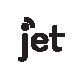
\includegraphics{logo_first_page}}  
	\put(30,-22){\scriptsize\MakeUppercase{INTL Journal of Electronics and Telecommunications, \YEAR, Vol. \VOLUME, no. \NUMBER, pp. \PAGES}}
	\put(30,-30){\scriptsize{Manuscript received \RECEIVEDATE; revised \REVISIONDATE.$\qquad\qquad\qquad$\DOI}}
	\end{picture}
}
\chead{}
\rhead{}
\lfoot
{
	\begin{picture}(0,0)
	\put(0,0){\doclicenseImage[imagewidth=5.5em]}  
	\put(65,12){\scriptsize $\copyright$ 
	{\scriptsize The Author(s). This is an open-access article distributed under the terms of the Creative Commons Attribution License (CC BY 4.0,}}
	\put(65,2){\scriptsize {\href{https://creativecommons.org/licenses/by/4.0/}{https://creativecommons.org/licenses/by/4.0/}), which permits use, distribution, and reproduction in any medium, provided that the Article is properly cited.}}
	\end{picture}}

\cfoot{}
\rfoot{}
\renewcommand{\headrulewidth}{0pt}
\renewcommand{\footrulewidth}{0pt}

% added by author
\usepackage{tabularray}


%\begin{multicols}{1}
%\fancyfoot[L]{\doclicenseImage[imagewidth=4em] $\copyright$ 
%	{\scriptsize The Author(s). This is an open-access article distributed under the terms of the Creative Commons Attribution License (CC BY 4.0, \href{https://creativecommons.org/licenses/by/4.0/}{https://creativecommons.org/licenses/by/4.0/}), which permits use, distribution, and reproduction in any medium, provided that the Article is properly cited.}}
%\pagestyle{fancy}
%\end{multicols}

\setcounter{page}{300}

%\linespread{1.02}

%%%%%%%%%%%%%%%%%%%%%%%%%%%%%%%%%%%%%%%%%%%%%%%%%%%%%%%%%%%%%%%%%%%%%%%%%%%%%%%%%%%%%%%%%%%%%%%%%%%%%%%%%%%%%%%%%%%%%%%%%%%%%
%%%%%%%%%%%%%%%%%%%%%%%%%%%%%%%%%%%%%%%%%%%%%%%%%%%%%%%%%%%%%%%%%%%%%%%%%%%%%%%%%%%%%%%%%%%%%%%%%%%%%%%%%%%%%%%%%%%%%%%%%%%%%
% AUTHOR SECTION ( This is a skeleton file demonstrating the use of TEMPLATE_article_for_IJET_jrnl.tex)

%%pdfinfo is document information - this information makes pdf much more usefull for search engines;
%%clik ctr+D on open pdf document and check information about this document

\pdfinfo {
	/Author (Paweł Antoniuk, Sławomir Krzysztof Zieliński)
	/Title (Assessing Models for Estimation Ensemble Width in Binaural Music Recordings: Robustness to Reverberation and Noise)
	/Keywords (binaural audio, ensemble width, audio perception, localization, reverberation, machine learninge)
}

\hypersetup
{pdfauthor={Paweł Antoniuk, Sławomir Krzysztof Zieliński},%
pdftitle={Assessing Models for Estimation Ensemble Width in Binaural Music Recordings: Robustness to Reverberation and Noise},%
pdfsubject={International Journal of Electronics and Telecommunications, 4 (2022), 300-306. DOI: 10.24425/ijet.2022.139xxx},%
pdfkeywords={binaural audio, ensemble width, audio perception, localization, reverberation, machine learning},%
pdfproducer={LaTeX},%
pdfcreator={pdfLaTeX}
}
%%%%%%%%%%%%%%%%%%%%%%%%%%%%%%%%%%%%%%%%%%%%%%%%%%%%%%%
% BODY OF THE ARTICLE

\begin{document}

%
% paper title
% can use linebreaks \\ within to get better formatting as desired

\title{\vspace{1cm} Assessing Models for Estimation Ensemble Width in Binaural Music Recordings: \\ Robustness to Reverberation and Noise}
%
%
% author names and IEEE memberships
% note positions of commas and nonbreaking spaces ( ~ ) LaTeX will not break
% a structure at a ~ so this keeps an author's name from being broken across
% two lines.
% use \thanks{} to gain access to the first footnote area
% a separate \thanks must be used for each paragraph as LaTeX2e's \thanks
% was not built to handle multiple paragraphs
%

\author{Paweł~Antoniuk and Sławomir~Krzysztof~Zieliński% <-this % stops a space
\thanks{The work was supported by grants from Bialystok University of Technology (WI/WI-IIT/3/2022 and WZ/WI-IIT/5/2023) and funded with resources for research by the Ministry of Science and Higher Education in Poland.}% stops a space
\thanks{P.~Antoniuk and S. K. Zieliński are with Faculty of Computer Science, Bialystok University of Technology, Poland (e-mail: pawel.antoniuk@sd.pb.edu.pl, s.zielinski@pb.edu.pl).}% <-this % stops a space
}

% note the % following the last \IEEEmembership and also \thanks -
% these prevent an unwanted space from occurring between the last author name
% and the end of the author line. i.e., if you had this:
%
% \author{....lastname \thanks{...} \thanks{...} }
%                     ^------------^------------^----Do not want these spaces!
%
% a space would be appended to the last name and could cause every name on that
% line to be shifted left slightly. This is one of those \L{}aTeX things". For
% instance, "\textbf{A} \textbf{B}" will typeset as \k{A} B" not \k{A}B". To get
% \k{A}B" then you have to do: "\textbf{A}\textbf{B}"
% \thanks is no different in this regard, so shield the last } of each \thanks
% that ends a line with a % and do not let a space in before the next \thanks.
% Spaces after \IEEEmembership other than the last one are OK (and needed) as
% you are supposed to have spaces between the names. For what it is worth,
% this is a minor point as most people would not even notice if the said evil
% space somehow managed to creep in.



% The paper headers
%\markboth{Journal of \LaTeX\ Class Files,~Vol.~6, No.~1, January~2007}%
%{Shell \MakeLowercase{\textit{et al.}}: Bare Demo of IEEEtran.cls for Journals}%
%
\markboth{}{}
%
% The only time the second header will appear is for the odd numbered pages
% after the title page when using the twoside option.
%
% *** Note that you probably will NOT want to include the author's ***
% *** name in the headers of peer review papers.                   ***
% You can use \ifCLASSOPTIONpeerreview for conditional compilation here if
% you desire.




% If you want to put a publisher's ID mark on the page you can do it like
% this:
%\IEEEpubid{0000--0000/00\$00.00~\copyright~2007 IEEE}
% Remember, if you use this you must call \IEEEpubidadjcol in the second
% column for its text to clear the IEEEpubid mark.



% use for special paper notices
%\IEEEspecialpapernotice{(Invited Paper)}

%IJET header for even and odd pages (Caution: with exeption the first page)
\maketitle

\thispagestyle{fancy}\markboth{P.~Antoniuk, S.~K.~Zieliński}{Assessing Models for Estimation Ensemble Width in Binaural Music Recordings: Robustness to Reverberation and Noise}
%


% ABSTRACT
 
\begin{abstract}
  Binaural technology has been known for decades. However, advancements in software and consumer electronics have facilitated its widespread adoption, primarily in the post-millennium era. As binaural sound becomes more popular, the demand for spatial analysis tools is expected to grow. This paper evaluates three methods for assessing ensemble width in binaural music recordings: (1) an auditory model with decision trees, (2) a~neural network model, and (3) a spatial spectrogram approach. Under ideal, anechoic conditions, the auditory model performed best with a~mean absolute error (MAE) of 6.59\textdegree{} (\textpm 0.11\textdegree{}), followed by the neural network (8.57\textdegree{} \textpm 0.19\textdegree{}) and the technique based on spatial spectrograms (13.54\textdegree{} \textpm 0.92\textdegree{}). Extending previous work, this study analyzes the methods' robustness to reverberation and noise. Noise resilience tests indicate moderate resistance, with the~auditory model yielding an MAE of 12.34\textdegree{} at a 10 dB signal-to-noise ratio. However, reverberation tests show a significant drop in accuracy even at an RT60 reverberation time of 0.1 seconds. The findings may contribute to the improvement of models for estimating ensemble width in binaural recordings of music, which could influence the development of binaural sound analysis tools, with potential applications in audio production.
\end{abstract}


% KEYWORDS 

\begin{IEEEkeywords}
binaural audio, ensemble width, audio perception, localization, reverberation, machine learning
\end{IEEEkeywords}

\IEEEpeerreviewmaketitle

% FIRST section - INTRODUCTION 

\section{Introduction}


% The very first letter is a 2 line initial drop letter followed
% by the rest of the first word in caps.
%
% form to use if the first word consists of a single letter:
% \IEEEPARstart{A}{demo} file is ....
%
% form to use if you need the single drop letter followed by
% normal text (unknown if ever used by IEEE):
% \IEEEPARstart{A}{}demo file is ....
%
% Some journals put the first two words in caps:
% \IEEEPARstart{T}{his demo} file is ....
%
% Here we have the typical use of a "T" for an initial drop letter
% and "HIS" in caps to complete the first word.
\IEEEPARstart{T}{his} demo file is intended to serve as a ``starter file''
for IEEE journal papers produced under \LaTeX\ using
IEEEtran.cls version 1.7 and later.
% You must have at least 2 lines in the paragraph with the drop letter
% (should never be an issue)

Lorem ipsum dolor sit amet, consectetur adipiscing elit, sed do eiusmod tempor incididunt ut labore et dolore magna aliqua. Ut enim ad minim veniam, quis nostrud exercitation ullamco laboris nisi ut aliquip ex ea commodo consequat.  Duis aute irure dolor in reprehenderit in voluptate velit esse cillum dolore eu fugiat nulla pariatur. Excepteur sint occaecat cupidatat non proident, sunt in culpa qui officia deserunt mollit anim id est laborum \cite{Chitambar2019},\cite{CISCO2020}. Excepteur sint occaecat cupidatat non proident, sunt in culpa qui officia deserunt mollit anim id est laborum. See Fig.~\ref{fig:lena1}.
% FIGURE 
% An example of a floating figure using the graphicx package.
% Note that \label must occur AFTER (or within) \caption.
% For figures, \caption should occur after the \includegraphics.
% Note that IEEEtran v1.7 and later has special internal code that
% is designed to preserve the operation of \label within \caption
% even when the captionsoff option is in effect. However, because
% of issues like this, it may be the safest practice to put all your
% \label just after \caption rather than within \caption{}.
%
% Reminder: the "draftcls" or "draftclsnofoot", not "draft", class
% option should be used if it is desired that the figures are to be
% displayed while in draft mode.
%
%\begin{figure}[!t]
%\centering
%\includegraphics[width=2.5in]{myfigure}
% where an .eps filename suffix will be assumed under latex,
% and a .pdf suffix will be assumed for pdflatex; or what has been declared
% via \DeclareGraphicsExtensions.
%\caption{Simulation Results}
%\label{fig_sim}
%\end{figure}

% Note that IEEE typically puts floats only at the top, even when this
% results in a large percentage of a column being occupied by floats.


% An example of a double column floating figure using two subfigures.
% (The subfig.sty package must be loaded for this to work.)
% The subfigure \label commands are set within each subfloat command, the
% \label for the overall figure must come after \caption.
% \hfil must be used as a separator to get equal spacing.
% The subfigure.sty package works much the same way, except \subfigure is
% used instead of \subfloat.
%
%\begin{figure*}[!t]
%\centerline{\subfloat[Case I]\includegraphics[width=2.5in]{subfigcase1}%
%\label{fig_first_case}}
%\hfil
%\subfloat[Case II]{\includegraphics[width=2.5in]{subfigcase2}%
%\label{fig_second_case}}}
%\caption{Simulation results}
%\label{fig_sim}
%\end{figure*}
%
% Note that often IEEE papers with subfigures do not employ subfigure
% captions (using the optional argument to \subfloat), but instead will
% reference/describe all of them (a), (b), etc., within the main caption.

\begin{figure}[htbp]
	\begin{center}
		a) 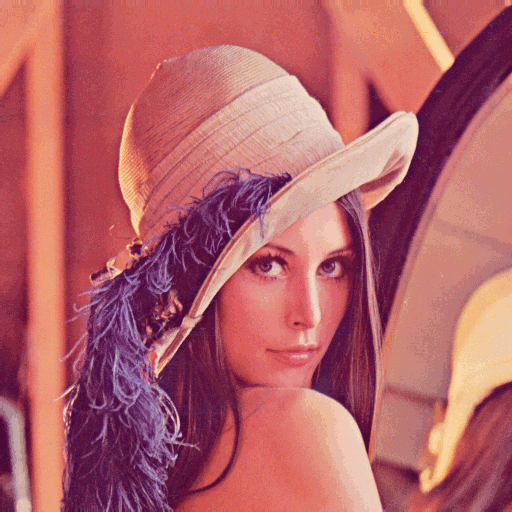
\includegraphics[width=0.4\linewidth]{img/lena.png} 
		b) 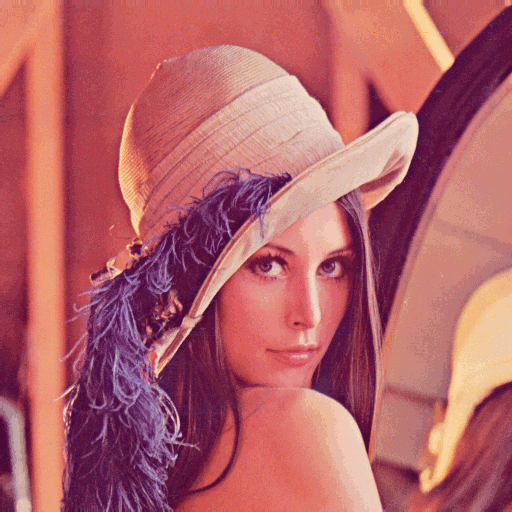
\includegraphics[width=0.4\linewidth]{img/lena.png} 
	\end{center}
	\caption{Exemplary image of Lena} \label{fig:lena1}
\end{figure}

computational coprocessors in classical ICT systems, but so far only for a confined set of problems~\cite{Preskill2018}. Search goes on widening this set.


%Related Studies
\section{Related Studies}

Estimating ensemble width represents a unique approach within binaural audio literature, which more commonly focuses on identifying the locations of individual sound sources \cite{benaroya_binaural_2018,ma_speech_2016,ma_exploiting_2017,may_probabilistic_2011,may_robust_2015}. While analyzing individual sound sources might seem more useful because it yields more precise information, such methods have limitations that hinder their practical application. These include a limited or predetermined number of sound sources and a predetermined type of audio signal—typically speech \cite{benaroya_binaural_2018,ma_speech_2016,may_probabilistic_2011,may_robust_2015,yang_deepear_2024}. The ensemble approach serves as a workaround for these limitations by providing useful spatial information without such constraints.

Traditional audio localization methods often rely on arrays with more than two microphones to improve precision through additional channel information \cite{pavlidi_real-time_2012,hahmann_sound_2022,liu_sound_2022}. While adding microphones can enhance precision through additional channel information, they do not utilize binaural hearing principles, rendering them ineffective for binaural recording assessment. By contrast, as Yang et al. demonstrate, systems using only two microphones can achieve superior localization accuracy by integrating binaural cues \cite{yang_deepear_2024}.

The majority of studies on sound source localization in binaural recordings concentrate on the localization of individual sources in isolation, typically referred to as Direction of Arrival (DoA) \cite{benaroya_binaural_2018,ma_speech_2016,ma_exploiting_2017,may_probabilistic_2011,may_robust_2015}. Although this granular approach provides detailed information, the existing methods require \textit{a~priori} knowledge of the number of sources, usually limiting analysis to between one and six sources. These constraints present significant challenges in real-life scenarios, where such advance knowledge is unavailable. Moreover, these methods have been developed primarily for homogeneous signals, especially speech, making them impractical for real-world binaural recordings where signals are often heterogeneous.

In a series of recent studies, Arthi and Sreenivas \cite{arthi_binaural_2022}, Antoniuk at al. \cite{antoniuk_blind_2023,antoniuk_ensemble_2024,antoniuk_estimating_2024}, introduced an alternative approach, treating sound sources as ensembles that can be characterized by their location and width, as illustrated in Figure \ref{fig:figx}. This method overcomes the limitations of traditional DoA approaches by focusing on ensemble characteristics rather than precise individual source locations. The approach eliminates the need for \textit{a prior} knowledge of the number of sources and has been validated across diverse musical content, including both instrumental and vocal recordings \cite{antoniuk_blind_2023,antoniuk_ensemble_2024,antoniuk_estimating_2024}.

\begin{figure}[htbp]
	\begin{center}
		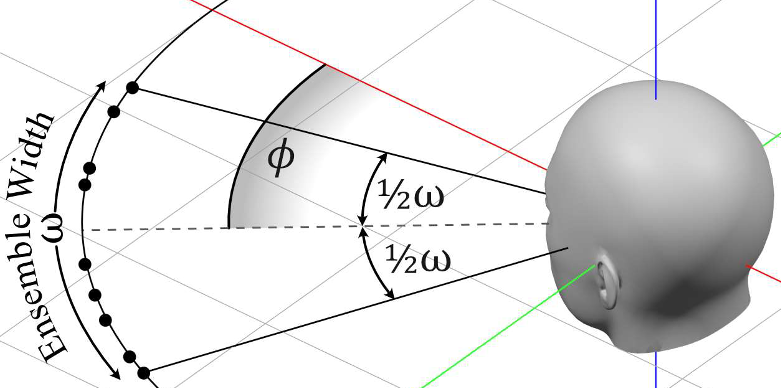
\includegraphics[width=1.0\linewidth]{img/figx.png} 
	\end{center}
	\caption{An ensemble example comprising nine point-like sound sources shown as dots. The ensemble's width is denoted by $\omega$, while $\phi$ indicates the counterclockwise position of the ensemble's center.} \label{fig:figx}
\end{figure}

This approach aligns with the second level of Rumsey's spatial audio scene-based framework \cite{rumsey_spatial_2002}, which defines three distinct levels: (1) single source, (2) scene, and (3) environment. Scene-level analysis, as described by Rumsey, better matches the human auditory system's natural source-grouping mechanisms. The approach mirrors real-world musical performance configurations where instruments and vocals occupy adjacent spatial positions. Notably, the methods incorporated in this study specifically measure physical ensemble width rather than apparent ensemble width---two related but distinct parameters whose relationship warrants further investigation.


%Methodology
\section{Methodology}

This study compares three recent methods for ensemble width estimation:
\begin{enumerate}
    \item a method based on an auditory model and decision trees (Section \ref{sec:methods:auditory}),
    \item a method using deep neural network (Section \ref{sec:methods:neural}),
    \item a method leveraging spatial spectrograms (Section \ref{sec:methods:spatial}).
\end{enumerate}
Initially, these methods were evaluated using anechoic recordings without noise. To test their performance in more ecological conditions, the methods were also tested using signals with predefined signal-to-noise ratios and simulated rooms with different reverberation characteristics (see Section \ref{sec:environmental}).

The objective of the methods incorporated in this study is to estimate the ensemble width ($\omega$) as illustrated in Figure \ref{fig:figx}. An ensemble is defined as a group of audio point sources positioned equidistantly around the listener on a circular virtual acoustic scene. The location of source $i$ is denoted by $\theta_i$. The~ensemble width ($\omega$) represents the angular distance between the two extreme point sources $(\max_i(\theta_i) - \min_i(\theta_i))$, while the ensemble location, represented by $\phi$, indicates the~midpoint angle between these extreme sources $((\max_i(\theta_i) + \min_i(\theta_i)) / 2)$. In this study, source locations are restricted to the frontal hemisphere, specifically $\theta \in [-45\degree, 45\degree]$ and $\omega \in [0\degree, 90\degree]$. It should be noted that although humans have some limited abilities to localize sound sources in the vertical plane, all sources in this study are positioned on the horizontal plane at ear level. These constraints reflect most real-world recording scenarios.


% % EQUATION 

% \begin{equation} \label{eq:1}
% \alpha + \beta = \gamma
% \end{equation}

% \subsection{Subsection Heading Here}
% Lorem ipsum dolor sit amet, consectetur adipiscing elit, sed do eiusmod tempor incididunt ut labore et dolore magna aliqua. Ut enim ad minim veniam, quis nostrud exercitation ullamco laboris nisi ut aliquip ex ea commodo consequat. Duis aute irure dolor in reprehenderit in voluptate velit esse cillum dolore eu fugiat nulla pariatur. Excepteur sint occaecat cupidatat non proident, sunt in culpa qui officia deserunt mollit anim id est laborum:

% \begin{itemize}
% 	\item one,
% 	\item two,
% 	\item three.
% \end{itemize}

% Lorem ipsum dolor sit amet, consectetur adipiscing elit, sed do eiusmod tempor incididunt ut labore et dolore magna aliqua. Ut enim ad minim veniam, quis nostrud exercitation ullamco laboris nisi ut aliquip ex ea commodo consequat. Duis aute irure dolor in reprehenderit in voluptate velit esse cillum dolore eu fugiat nulla pariatur. Excepteur sint occaecat cupidatat non proident, sunt in culpa qui officia deserunt mollit anim id est laborum. See Fig. \ref{fig:fig2}.

% \begin{figure}[htbp]
% 	\begin{center}
% 		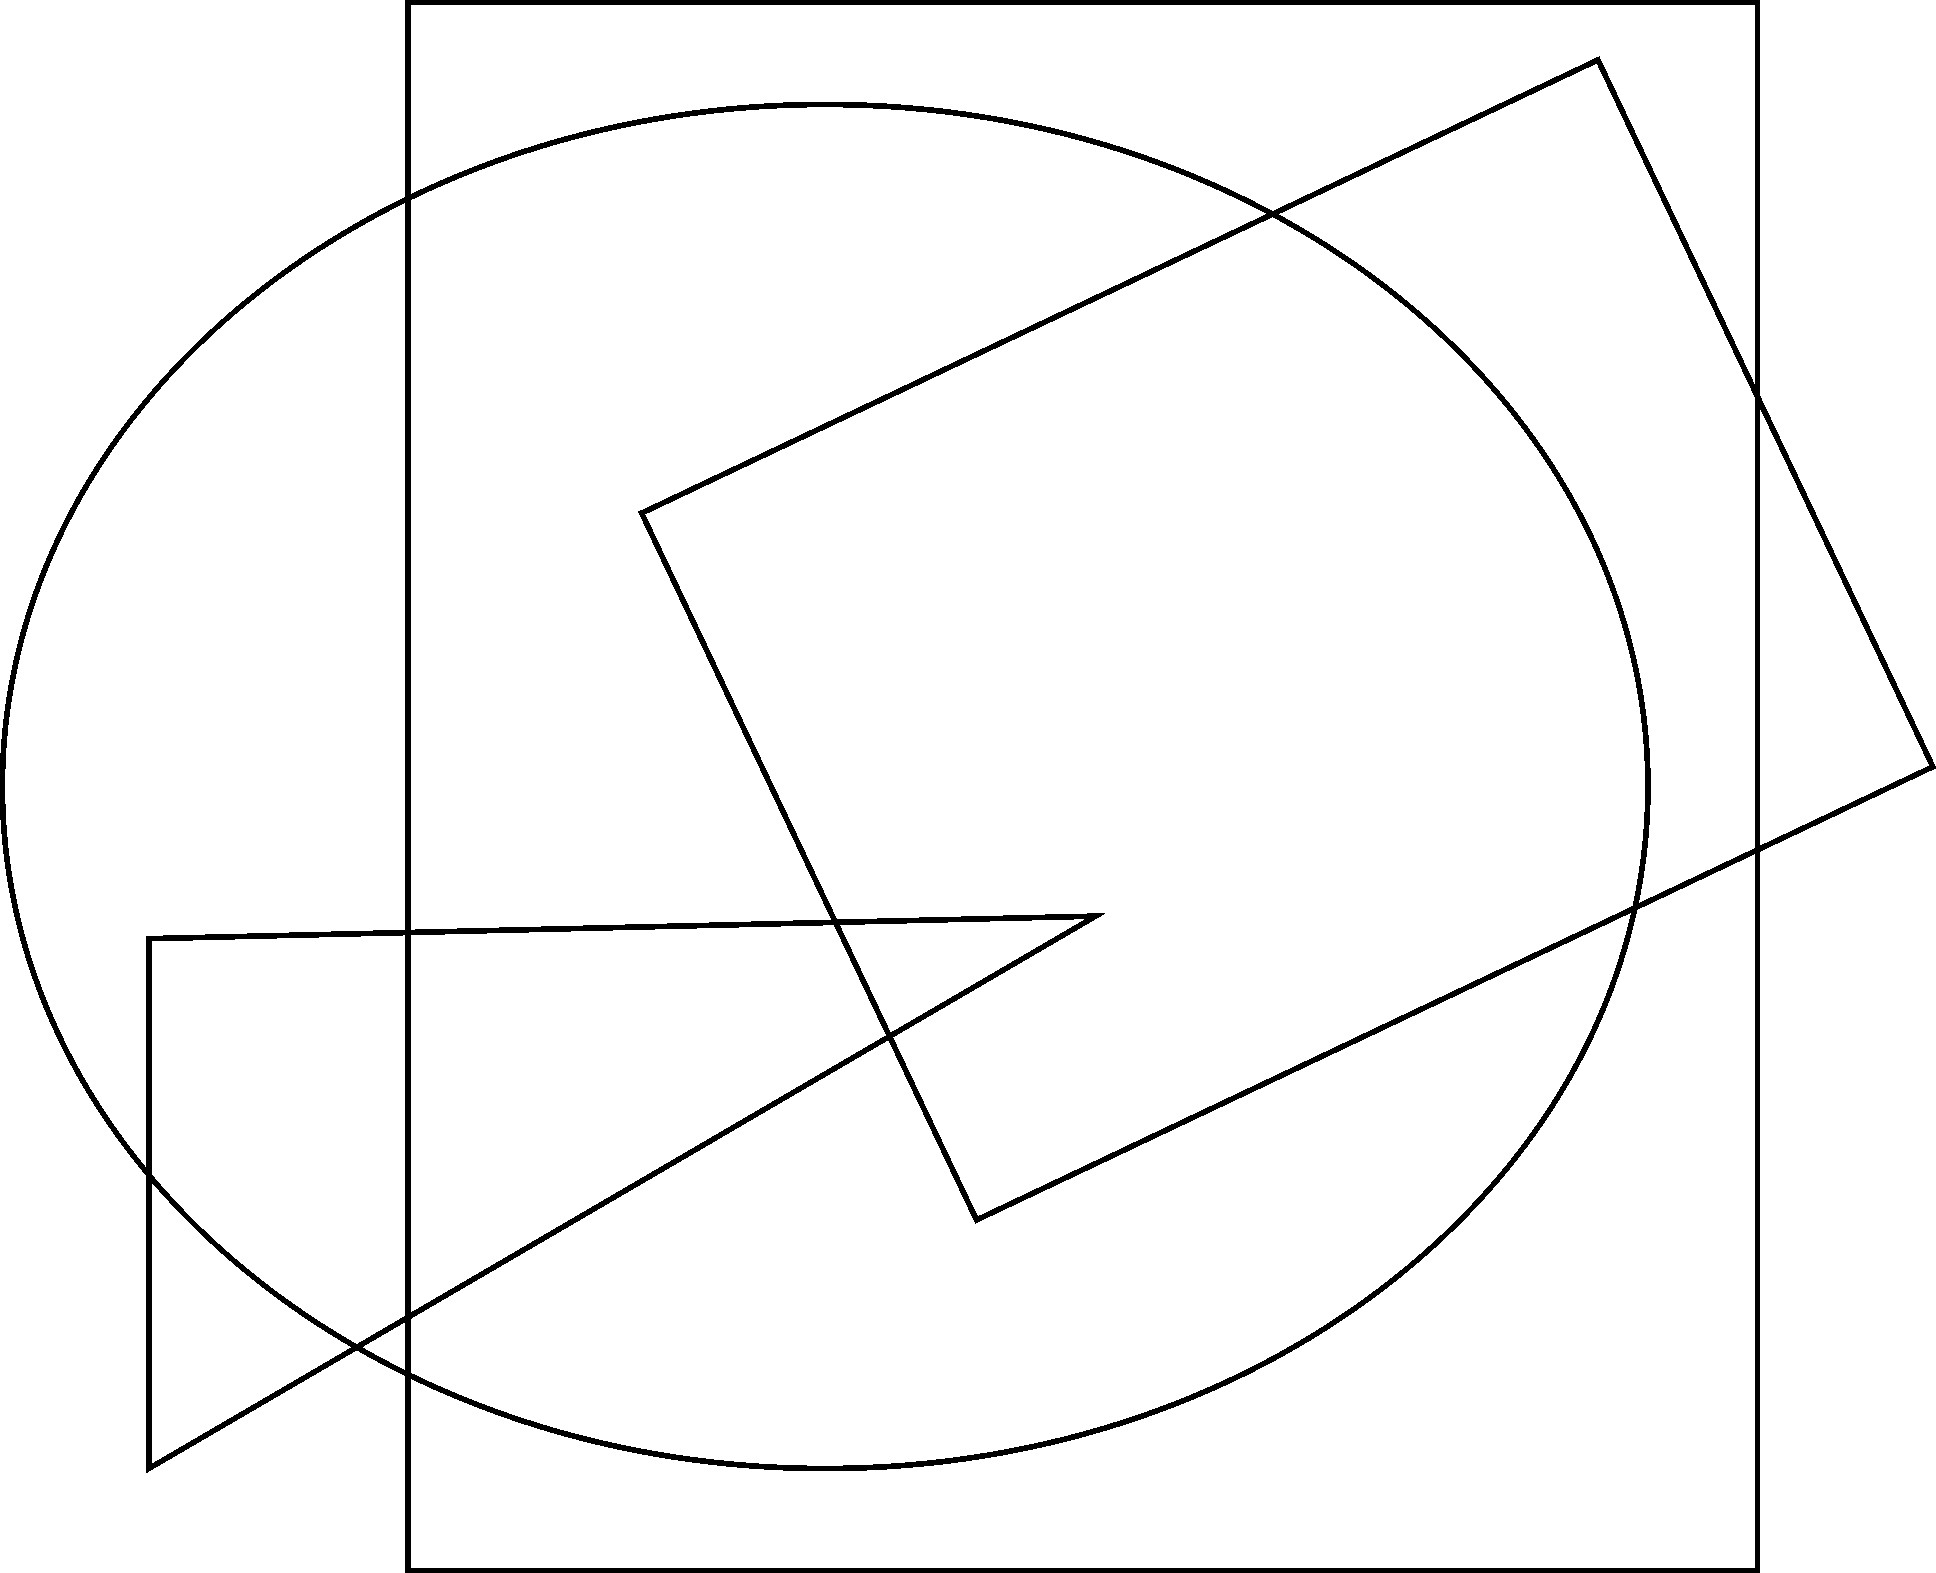
\includegraphics[width=0.8\linewidth]{img/fig2.jpg} 
% 	\end{center}
% 	\caption{Explain the significance of the figure in the caption} \label{fig:fig2}
% \end{figure}


%*****************************************



\section{Dataset Preparation}

The experimental evaluation was conducted using a corpus of 23,040 synthesized binaural music recordings. The source material comprised 192 publicly-available multi-track recordings spanning diverse musical genres including rock, jazz, pop, and classical music. The number of tracks ranged from 5 to 62, with a median of 9.

To ensure robust evaluation across diverse Head-Related Transfer Function (HRTF) characteristics, the synthesis process incorporated 30 HRTF databases (see Table \ref{table:hrtfs} in Appendix for a detailed list). These databases were evenly divided into measurements from human subjects (15 databases) and measurements from artificial heads (15 databases), including industry-standard devices such as the Neumann KU 100 and KEMAR DB-4004. Distances between the head and loudspeaker during HRTF measurements ranged from 0.9 to 1.95 meters, with a median of 1.2 meters.

For each combination of multi-track recording and HRTF database, four unique binaural versions were synthesized by randomly varying two ensemble parameters: location ($\phi$) and width ($\omega$). Within these spatial constraints, individual tracks in each recording were randomly assigned to specific source positions ($\theta_i$). Prior to synthesis, all tracks were loudness-normalized to -23~LKFS in accordance with ITU-R BS.1770-5 recommendations \cite{noauthor_itu-r_2023}, ensuring consistent relative levels across the corpus.

Multiple HRTFs and multi-track recordings were selected to create diverse binaural recordings, enhancing the model's generalisability. This diversity is crucial for HRTFs since the~specific HRTF used in real-world binaural synthesis is often unknown, making a single-HRTF model impractical for general use. Additionally, the large dataset provides essential training material for all machine learning models used in this study, with particular importance for the deep neural networks, as their performance benefits significantly from extensive data.

The binaural recordings were obtained using a binauralization procedure, implemented by convolving multi-track signals with head-related impulse responses from a specified HRTF database. The resulting binaural output signal, $y_c[n]$, for each stereo channel $c$ (left or right) at sample $n$ is given by the~following equation:
\begin{equation} \label{eq:1}
    y_c[n] = \sum_{i=1}^{N} \sum_{k=0}^{K-1} x_i[k] \times h_{c,\theta_i}[n-k],
\end{equation}
where $x_i$ denotes the signal of an individual sound source $i$ from the input music recording, and  $h_{c,\theta_i}$ represents the head-related impulse response for channel $c$ at location $\theta_i$ of source track $i$. Additionally, $N$ denotes the number of track sources in the~input multi-track recording, and $K$ represents the number of samples in the recording.

The synthesized recordings were truncated to 7 seconds following binauralization, with sine-squared fade-in and fade-out effects of 0.01 seconds applied. Subsequently, the signals were RMS-normalized, scaled by a factor of 0.9, DC-offset corrected, and stored as uncompressed files with a sample rate of 48 kHz and 32-bit resolution.

The binaural recordings were randomly split into training and test sets with a 2:1 ratio. To prevent information `leakage', this split was made in such a way that no multi-track recordings used for training were used for testing. To reduce the~complexity of the experiment, the HRTFs were shared between both sets, which could be seen as a limitation of this study. However, it is known that the human auditory system operates with HRTFs that undergo only minimal changes throughout life, mainly during infancy \cite{king_how_2001}. Therefore, this limitation could be considered consistent with how the human auditory system behaves in real life. 

The binauralization and split procedures implemented in this study are consistent with those originally described in the reference models \cite{antoniuk_blind_2023,antoniuk_ensemble_2024,antoniuk_estimating_2024}, with minor modifications. The~primary modification pertains to the spatial-spectrogram-based model, which utilized a single HRTF database and employed a~reduced parameter set. This modification had minimal impact on the results, as the method employs a deterministic approach rather than machine learning techniques, requiring the training set only for the optimization of two parameters.


\section{Auditory-Model-Based Method}
\label{sec:methods:auditory}

As shown in Figure \ref{fig:fig3}, the auditory-model-based method for ensemble width estimation consists of two main components: a binaural auditory model that extracts features from the input signals, followed by a gradient-boosted decision tree regressor that predicts the ensemble width \cite{antoniuk_ensemble_2024}. The auditory model processes the binaural signals through a gammatone filterbank and extracts standard binaural cues, including interaural time differences (ITD), interaural level differences (ILD), and interaural cross-correlation (IACC).

\begin{figure}[htbp]
	\begin{center}
		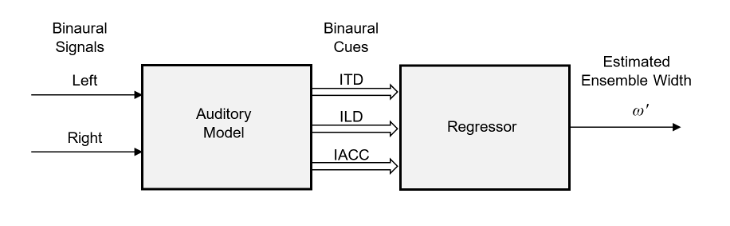
\includegraphics[width=1.0\linewidth]{img/auditory_flowchart.png} 
	\end{center}
	\caption{A flowchart of the auditory-model-based method \cite{antoniuk_ensemble_2024}} \label{fig:fig3}
\end{figure}

The auditory model is based on the work of S{\o}ndergaard and Majdak~\cite{blauert_technology_2013}, enhanced by May et al.~\cite{may_probabilistic_2011}, and further refined by Decorsi{\`e}re and May~\cite{decorsiere_auditory_2016} within Two!Ears Project~\cite{raake_computational_2016}. The~model consists of a gammatone filterbank with 64 frequency channels spanning from 100~Hz to 16~kHz. For each frequency channel, the inner hair-cell envelopes are extracted through half-wave rectification followed by low-pass filtering using a second-order Butterworth filter with a~1~kHz cutoff frequency. This simulates the loss of phase-locking in the~auditory nerve at higher frequencies. Rate maps, representing auditory nerve firing rates, are then calculated by smoothing the inner hair-cell signal with a~leaky integrator (time constant of 8~ms) and averaging within 20~ms Hann-windowed frames with 10~ms step size. Finally, the rate maps were used to estimate the binaural cues.

The features extracted in the~previous component are aggregated across time-frames by computing their mean values and standard deviations, resulting in a total of 384 feature vectors (64 frequency channels $\times$ 3 types of cues $\times$ 2 statistics). These aggregated features are then used as input to the~regressor, whose objective is to estimate the ensemble width of the binaural audio signal. The~regressor employs gradient-boosted decision trees implemented with LightGBM, known for its computational efficiency and accuracy \cite{ke_lightgbm_2017}. The~model's hyperparameters---including the number of leaves, tree depth, and learning rate---were optimized using grid search procedure. The final training was conducted using validation set and early-stopping technique based on mean absolute error. For further details, see~\cite{antoniuk_ensemble_2024}.


\section{Neural-Network-Based Method}
\label{sec:methods:neural}

While the auditory-model-based method attempts to mimic human hearing mechanisms, the neural network approach takes advantage of Convolutional Neural Networks (CNNs) and their ability to automatically learn relevant features from spectral representations of audio signals. In contrast to the~auditory-model-based approach, the neural network method uses a basic feature extraction technique based on magnitude spectrograms \cite{antoniuk_estimating_2024}.

A Hamming window of 40 ms with an~overlap of 20 ms is applied, resulting in 349 time frames extracted for each binaural input signal. For each time frame, the Fast Fourier Transform (FFT) is applied. The magnitudes of its output are aggregated into 64 linearly spaced frequency bands ranging from 100 Hz to 16 kHz, effectively creating a spectrogram with dimensions $349 \times 64$. This process is performed separately for the left and right channels, producing a pair of spectrograms that are then used in the neural network to simultaneously estimate two ensemble parameters: width and location. However, only ensemble width is considered in this study.

In the next step, the spectrograms are input into a two-dimensional CNN model to estimate the ensemble width, effectively treating the spectrograms as visual data. The network's topology is based on the AlexNet model introduced by Krizhevsky et al.~\cite{krizhevsky_imagenet_2017}. The input layer is followed by five convolutional units, each consisting of a ReLU-activated 2D convolution layer with a~$2 \times 2$ filter size, followed by a~max pooling layer of size $2 \times 3$ or $2 \times 2$. The number of convolutional filters in each layer is 32, 64, 128, and 256, respectively. Following these layers, a global average pooling layer is applied to reduce overfitting \cite{lin_network_2013}. The next stage consists of four fully connected layers with ReLU activation, reducing the activation map's dimensions from 256 to 6. Finally, two parallel fully connected layers with linear activation are used to predict the ensemble parameters; one outputs the~ensemble width, and the other outputs the~ensemble location.

In total, this topology resulted in a model with 216,562 learning parameters. The model was trained using a Monte Carlo cross-validation procedure with 10 repetitions and an~early-stopping validation subset. For further details, see~\cite{antoniuk_estimating_2024}.


\section{Spatial-Spectrogram-Based Method}
\label{sec:methods:spatial}

The spatial-spectrogram-based method, originally introduced by Arthi and Sreenivas \cite{arthi_binaural_2022}, employs a phase-only spatial correlation (POSC) function to estimate ensemble width, treating the binaural signals primarily in the frequency domain. The~method consists of three main steps: calculation of generalized cross-correlation functions, generation of spatial spectrograms, and ensemble width estimation.

First, two generalized cross-correlation functions with phase transform (GCC-PHAT) are calculated:
\begin{equation}
\rho(k) \stackrel{\mathcal{F}}{\longleftrightarrow} \frac{X_r(\omega) \times X_l^*(\omega)}{|X_r(\omega) \times X_l^*(\omega)|},
\end{equation}
\begin{equation}
\rho_\theta(k) \stackrel{\mathcal{F}}{\longleftrightarrow} \frac{H_r^\theta(\omega) \times H_l^{\theta*}(\omega)}{|H_r^\theta(\omega) \times H_l^{\theta*}(\omega)|},
\end{equation}
where $\rho(k)$ denotes the GCC-PHAT function for the \mbox{$k$-th} sample of the binaural signal; $\rho_\theta(k)$ represents the GCC-PHAT function for the $k$-th sample of the HRIR; $X_l(\omega)$ and $X_r(\omega)$ are Fourier transforms of the~left and right channel signals, respectively; $H_l^\theta$ and $H_r^\theta$ are Fourier transforms of the~left and right channels, respectively, for the HRIR at azimuth $\theta$; and~$^*$~denotes complex conjugate. The phase-only spatial correlation (POSC) function $C_\rho(\theta)$ is then calculated as:

\begin{equation}
C_\rho(\theta) \triangleq \sum \rho(k) \times \rho_\theta(k)
\end{equation}

To account for the observation that sources closer to $0\degree$ have a greater impact on $C_\rho(\theta)$ than more distant sources, a~correction is applied:

\begin{equation}
\widetilde{C_\rho(\theta)} = C_\rho(\theta) \times (1 + \theta u),
\end{equation}
where $u$ is a correction weight determined through optimization.

The ensemble width is estimated using a three-step algorithm:

\begin{enumerate}
\item Find $\max \widetilde{C_\rho(\theta)}$ considering all frames in the binaural excerpt.
\item Find the minimal ($\theta_a$) and maximal ($\theta_b$) roots of:
      \begin{equation}
      \widetilde{C_\rho(\theta)} = t_h \times \max \widetilde{C_\rho(\theta)},
      \end{equation}
      where $t_h \in [0,1]$ is a threshold coefficient.
\item Calculate ensemble width as $\omega = \theta_b - \theta_a$ averaged over all frames.
\end{enumerate}

The method requires optimization of only two parameters: the correction weight $u$ and threshold coefficient $t_h$. These parameters are determined using a grid search procedure with $u \in [0,2]$ and $t_h \in [0,1]$. Unlike the previous two methods, this approach is deterministic and does not require extensive training data, making it computationally efficient but potentially less accurate. For further details, see~\cite{antoniuk_blind_2023}.

% \begin{figure}[t]
% \centering
% \includegraphics[width=0.9\linewidth]{spatiogram_method}
% \caption{A flowchart of the spatial-spectrogram-based method illustrating the three main processing steps}
% \label{fig:spatiogram_method}
% \end{figure}


\section{Environmental Simulation}
\label{sec:environmental}

To enhance ecological validity, the original recording synthesis procedure was modified to enable evaluation under two additional scenarios: recordings with additive noise and recordings in reverberant conditions. In the first scenario, nine test sets were prepared with different Signal-to-Noise Ratios (SNR) ranging from -10 to 60 dB, specifically at -10, -3, 0, 10, 20, 30, 40, 50, and 60 dB. This was achieved by adding decorrelated white noise signals to the binaural recordings originally used in the testing procedure.

In the reverberation scenario, six different rooms were simulated with reverberation times ranging from 0.1 to 3 s, measured using the RT60 metric. The simulations were performed with MCRoomSim—a multichannel `shoebox' room acoustic simulator based on image source and diffuse rain algorithms implemented as a MATLAB package \cite{wabnitz_room_2010}. This simulator enabled the creation of reverberation simulations used to generate Binaural Room Impulse Responses (BRIRs) based on provided HRTFs, with the number of virtual speakers matching the~spatial density of measurement points in the~HRTF database. The virtual listener, modeled as a head with two receivers representing ears, was positioned in the~center of the room. The receivers were configured to filter the input signal directionally using head-related impulse responses from the given HRTF database. The distance between each virtual impulse source and the head center matched the measurement radius of the given HRTF database, ranging from 0.9 to 1.95~m. The room reverberation characteristics were controlled by configuring the following parameters: room width and depth (2--5 m), height (2.5--5 m), wall absorption coefficients (0.05--0.95), and wall scattering coefficients (0.01--0.8).


%Experiment
\section{Results}

Under baseline anechoic, noise-free conditions, the method based on an auditory model (1) achieved the highest accuracy, with a Mean Absolute Error (MAE) of $6.59\degree$ ($\pm0.11\degree$). This was followed by the neural network-based method (2) at $8.57\degree$ ($\pm0.19\degree$) and the spatial-spectrogram-based method (3) at $13.54\degree$ ($\pm0.92\degree$). All differences between the methods were statistically significant ($p<0.01$).

Auditory-model-based (1) and neural-network-based methods (2) exhibited varying degrees of noise resilience (Figure~\ref{fig:snr}). The neural-network-based method (2) maintained reasonable performance down to $\mathrm{SNR}=-3\,\mathrm{dB}$, while the~method incorporating an auditory model and decision trees (1) required $\mathrm{SNR}>10\,\mathrm{dB}$ for comparable results. The spatial-spectrogram-based method (3) was the most sensitive to noise, requiring $\mathrm{SNR} \geq 60\,\mathrm{dB}$ to operate reliably. These differences were statistically significant, with $p<0.01$.

\begin{figure}[htbp]
	\begin{center}
		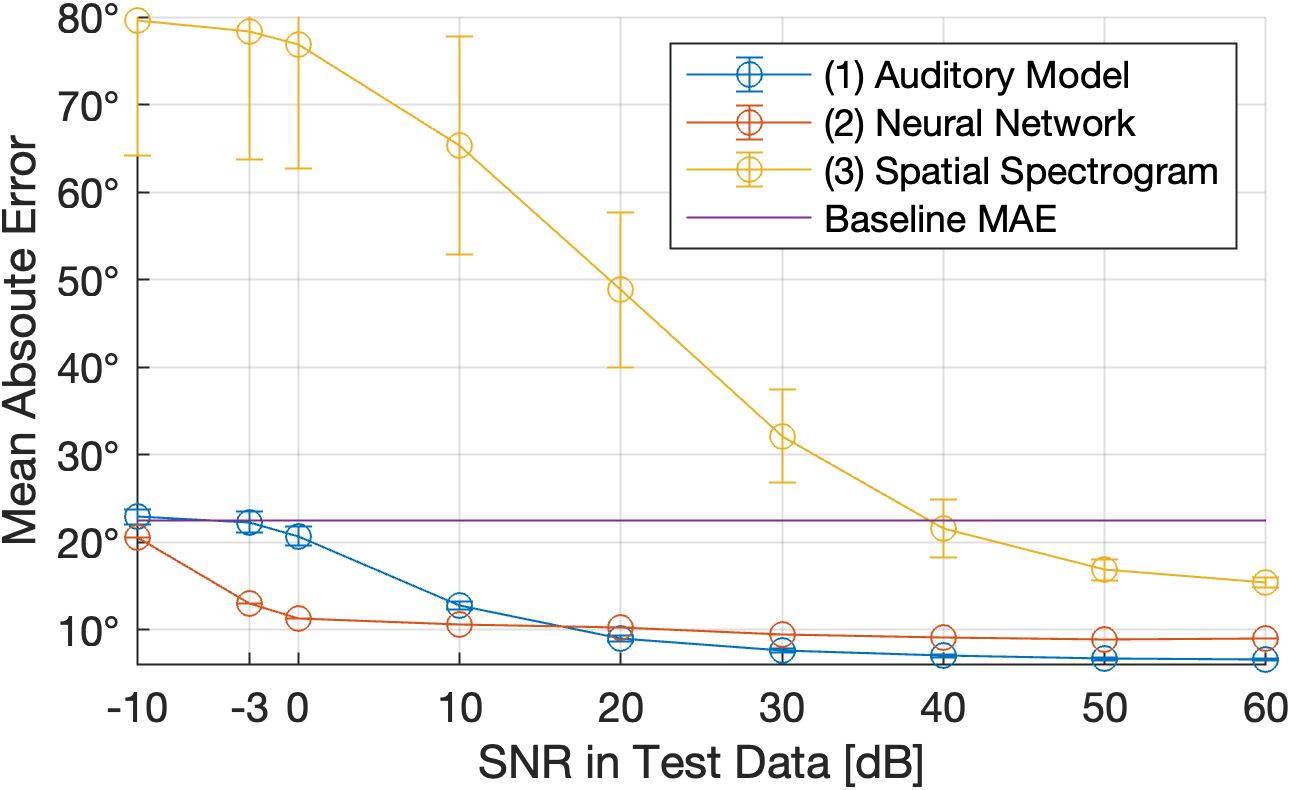
\includegraphics[width=1.0\linewidth]{img/mae_snr_full.png} 
	\end{center}
	\caption{Robustness to noise of the tested methods illustrating the mean absolute error (MAE) at varying signal-to-noise ratios (SNR). Error bars denote standard deviations. The baseline constant predictor (MAE = 22.5°) is included for comparison.} \label{fig:snr}
\end{figure}

Under reverberant conditions, all of the tested methods revealed significant limitations in performance (Figure \ref{fig:rt}). In~particular, the auditory-model-based method demonstrated notable difficulties even at minimal investigated reverberation times ($\mathrm{RT}{60}=0.1\,\mathrm{s}$). While all the methods outperformed the random baseline MAE at $\mathrm{RT}{60}=0.1\,\mathrm{s}$ ($p<0.01$), they demonstrated notable limitations. The primary cause seems to stem from their exclusive training on anechoic signals, leaving them ill-suited for the added temporal and spectral complexity of room reflections.

\begin{figure}[htbp]
	\begin{center}
		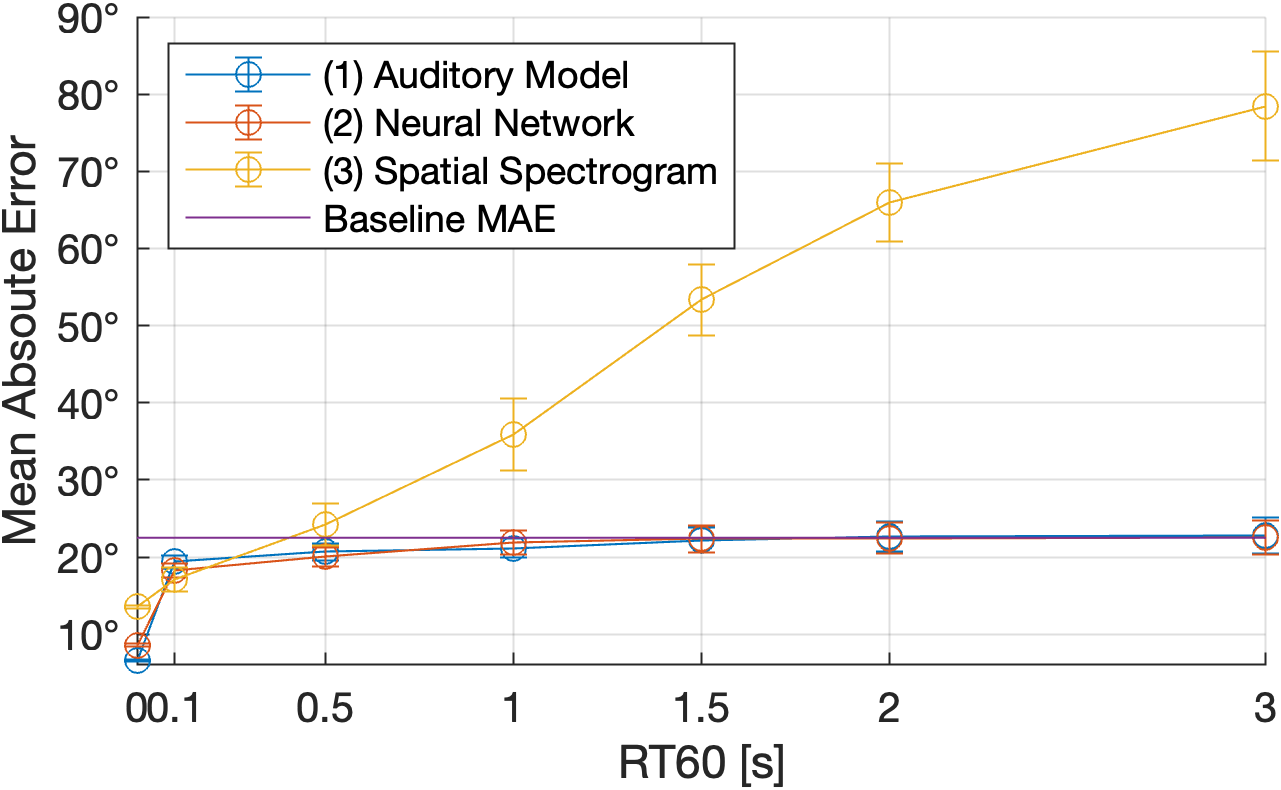
\includegraphics[width=1.0\linewidth]{img/mae_rt.png} 
	\end{center}
	\caption{Robustness to reverberation across tested models, shown as mean absolute error (MAE) for simulated rooms with varying RT60 values. Error bars denote standard deviations. The baseline constant predictor (MAE = 22.5°) is included for comparison.} \label{fig:rt}
\end{figure}

% \begin{figure}[htbp]
% 	\begin{center}
% 		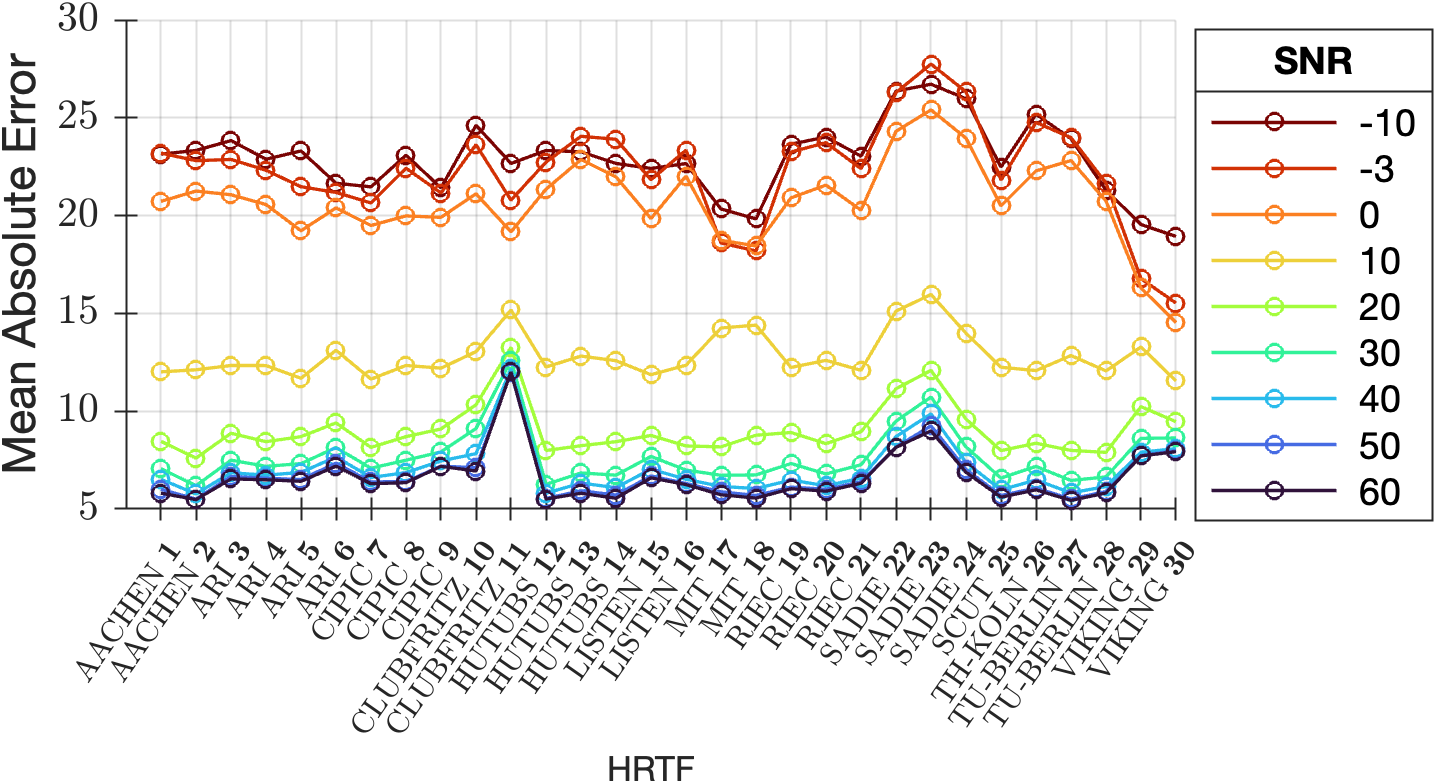
\includegraphics[width=1.0\linewidth]{img/mae_snr_hrtf.png} 
% 	\end{center}
% 	\caption{Mean absolute error (MAE) of ensemble width estimation across different HRTF databases at various signal-to-noise ratios (SNR). The plot demonstrates the varying robustness of the method across different HRTF measurements, with artificial head measurements (marked with *) generally showing more consistent performance compared to human head measurements.} \label{fig:snr_hrtf}
% \end{figure}


% TABLE 
% An example of a floating table. Note that, for IEEE style tables, the
% \caption command should come BEFORE the table. Table text will default to
% \footnotesize as IEEE normally uses this smaller font for tables.
% The \label must come after \caption as always.
%
%\begin{table}[!t]
%% increase table row spacing, adjust to taste
%\renewcommand{\arraystretch}{1.3}
% if using array.sty, it might be a good idea to tweak the value of
% \extrarowheight as needed to properly center the text within the cells
%\caption{An Example of a Table}
%\label{table_example}
%\centering
%% Some packages, such as MDW tools, offer better commands for making tables
%% than the plain LaTeX2e tabular which is used here.
%\begin{tabular}{|c||c|}
%\hline
%One & Two\\
%\hline
%Three & Four\\
%\hline
%\end{tabular}
%\end{table}


% Note that IEEE does not put floats in the very first column - or typically
% anywhere on the first page for that matter. Also, in-text middle ("here")
% positioning is not used. Most IEEE journals use top floats exclusively.
% Note that, LaTeX2e, unlike IEEE journals, places footnotes above bottom
% floats. This can be corrected via the \fnbelowfloat command of the
% stfloats package.


% \begin{table}[ht]
% 		\renewcommand{\arraystretch}{1.3}
% 	\caption{Results of simulation}
% 	\label{results}
% 	\centering
% 	\begin{tabular}{l|c|c|c|c}
% 		\hline\hline
% 		header & abc & ijk & xyz & $\theta$ \\
% 		\hline \hline
% 		one & 0.1 & 0.01 & 0.001 & 0.0001\\ 
% 		\hline
% 		two & 1.1 & 2.2 & 3.3 & 4.4\\
% 		\hline
% 		three & 1.1 & 2.2 & 3.3 & 4.4\\
% 		\hline\hline
% 	\end{tabular}
% \end{table}

% Lorem ipsum dolor sit amet, consectetur adipiscing elit, sed do eiusmod tempor incididunt ut labore et dolore magna aliqua. Ut enim ad minim veniam, quis nostrud exercitation ullamco laboris nisi ut aliquip ex ea commodo consequat. Duis aute irure dolor in reprehenderit in voluptate velit esse cillum dolore eu fugiat nulla pariatur. Excepteur sint occaecat cupidatat non proident, sunt in culpa qui officia deserunt mollit anim id est laborum.

% \subsection{Subsection Heading Here}
% Lorem ipsum dolor sit amet, consectetur adipiscing elit, sed do eiusmod tempor incididunt ut labore et dolore magna aliqua. Ut enim ad minim veniam, quis nostrud exercitation ullamco laboris nisi ut aliquip ex ea commodo consequat. Duis aute irure dolor in reprehenderit in voluptate velit esse cillum dolore eu fugiat nulla pariatur. Excepteur sint occaecat cupidatat non proident, sunt in culpa qui officia deserunt mollit anim id est laborum.

% % needed in second column of first page if using \IEEEpubid
% %\IEEEpubidadjcol

% \subsubsection{Subsubsection Heading Here}

% Lorem ipsum dolor sit amet, consectetur adipiscing elit, sed do eiusmod tempor incididunt ut labore et dolore magna aliqua. Ut enim ad minim veniam, quis nostrud exercitation ullamco laboris nisi ut aliquip ex ea commodo consequat (\ref{eq:2}).

% \begin{equation} \label{eq:2}
% 	\frac{{dP}}{{dt}} \approx \frac{{P_{k + 1}  - P_k }}{T}
% \end{equation}

% \subsubsection{Subsubsection Heading Here}

%  Duis aute irure dolor in reprehenderit in voluptate velit esse cillum dolore eu fugiat nulla pariatur. Excepteur sint occaecat cupidatat non proident, sunt in culpa qui officia deserunt mollit anim id est laborum.

% Lorem ipsum dolor sit amet, consectetur adipiscing elit, sed do eiusmod tempor incididunt ut labore et dolore magna aliqua. Ut enim ad minim veniam, quis nostrud exercitation ullamco laboris nisi ut aliquip ex ea commodo consequat. Duis aute irure dolor in reprehenderit in voluptate velit esse cillum dolore eu fugiat nulla pariatur. Excepteur sint occaecat cupidatat non proident, sunt in culpa qui officia deserunt mollit anim id est laborum.

% \subsection{Subsection Heading Here}
% Lorem ipsum dolor sit amet, consectetur adipiscing elit, sed do eiusmod tempor incididunt ut labore et dolore magna aliqua. Ut enim ad minim veniam, quis nostrud exercitation ullamco laboris nisi ut aliquip ex ea commodo consequat. Duis aute irure dolor in reprehenderit in voluptate velit esse cillum dolore eu fugiat nulla pariatur. Excepteur sint occaecat cupidatat non proident, sunt in culpa qui officia deserunt mollit anim id est laborum. Simulation times for each presented scenario are shown in Table~\ref{table_two}.

% \begin{table}[h]
% 	% increase table row spacing, adjust to taste
% 	\renewcommand{\arraystretch}{1.3}
% 	% if using array.sty, it might be a good idea to tweak the value of \\extrarowheight as needed to properly center the text within the cells
% 	\caption{Simulation times of each scenario}
% 	\label{table_two}
% 	\centering
% 	\begin{tabular}{l|c|c|c}
% 		\hline\hline
% 		& White~[s] & Black~[s] & White to Black\\
% 		\hline\hline
% 		scenario 1 & 5 & 15 & 3 x faster\\
% 		\hline
% 		scenario 2 & 3 & 21 & 7 x faster\\
% 		\hline
% 		scenario 3 & 4 & 24 & 6 x faster\\
% 		\hline
% 		scenario 4 & 7 & 56 & 8 x faster\\
% 		\hline
% 		scenario 5 & 10 & 120 & 12 x faster\\
% 		\hline
% 		scenario 6 & 12 & 24 & 2 x faster\\
% 		\hline\hline
% 	\end{tabular}
% \end{table}

% Lorem ipsum dolor sit amet, consectetur adipiscing elit, sed do eiusmod tempor incididunt ut labore et dolore magna aliqua. Ut enim ad minim veniam, quis nostrud exercitation ullamco laboris nisi ut aliquip ex ea commodo consequat. Duis aute irure dolor in reprehenderit in voluptate velit esse cillum dolore eu fugiat nulla pariatur. Excepteur sint occaecat cupidatat non proident, sunt in culpa qui officia deserunt mollit anim id est laborum.











\section{Conclusions}
% \textbf{TODO:}
%\begin{itemize}
%    \item All areas of QC are still currently in the phase of active research (far from being mature).
%    \item Both new and well-established technologies push the development of Quantum Devices further. 
%    \item The improvements of hardware and algorithms allow for emerging practical applications.
    
  Any comments and suggestions are welcomed so we can constantly improve this template to satisfy all authors’ research needs. 
    
\section{Conclusion}
Lorem ipsum dolor sit amet, consectetur adipiscing elit, sed do eiusmod tempor incididunt ut labore et dolore magna aliqua. Ut enim ad minim veniam, quis nostrud exercitation ullamco laboris nisi ut aliquip ex ea commodo consequat. Duis aute irure dolor in reprehenderit in voluptate velit esse cillum dolore eu fugiat nulla pariatur. Excepteur sint occaecat cupidatat non proident, sunt in culpa qui officia deserunt mollit anim id est laborum.

Lorem ipsum dolor sit amet, consectetur adipiscing elit, sed do eiusmod tempor incididunt ut labore et dolore magna aliqua. Ut enim ad minim veniam, quis nostrud exercitation ullamco laboris nisi ut aliquip ex ea commodo consequat. Duis aute irure dolor in reprehenderit in voluptate velit esse cillum dolore eu fugiat nulla pariatur. Excepteur sint occaecat cupidatat non proident, sunt in culpa qui officia deserunt mollit anim id est laborum.Lorem ipsum dolor sit amet, consectetur adipiscing elit, sed do eiusmod tempor incididunt ut labore et dolore magna aliqua \cite{Preskill2018}, \cite{Pontryagin1962,Shenoy2020,Shao2019,Kober2013}. Ut enim ad minim veniam, quis nostrud exercitation ullamco laboris nisi ut aliquip ex ea commodo consequat. Duis aute irure dolor in reprehenderit in voluptate velit esse cillum dolore eu fugiat nulla pariatur. Excepteur sint occaecat cupidatat non proident, sunt in culpa qui officia deserunt mollit anim id est laborum.


% if have a single appendix:
%\appendix[Proof of the Zonklar Equations]
% or
%\appendix  % for no appendix heading
% do not use \section anymore after \appendix, only \section*
% is possibly needed

% use appendices with more than one appendix
% then use \section to start each appendix
% you must declare a \section before using any
% \subsection or using \label (\appendices by itself
% starts a section numbered zero.)
%


%\appendices
%\section{Proof of the First Zonklar Equation}
%Appendix one text goes here.

% you can choose not to have a title for an appendix
% if you want by leaving the argument blank
%\section{}
%Appendix two text goes here.

%\end{itemize}

% % ACKNOWLEDGMENT 
% use section* for acknowledgement
\section*{Acknowledgment}

The authors would like to thank experts for their appropriate and constructive suggestions to improve this template.

%%REFERENCES
%\section{REFERENCES}
%\balance
%% REFERENCES
%
%\begin{thebibliography}{99}
%	\bibitem{smith2015} J. Smith, "Title of the paper", \emph{Journal name} 12 (3), 45--67 (2015).
%	\bibitem{young2015} M. Young, "The Technical Writer’s Handbook", Mill Valley, Toronto, 2015.
%	\bibitem{apostoli2012} P. Apostoli and A. Kanda, "Cantorian sets, fuzzy sets, rough sets and fregean sets", \emph{Bull. Pol. Ac.: Tech.} 50 (3), 247-276 (2012).
%	\bibitem{nicole} R. Nicole, "Title of paper with only first word capitalized", J. Name Stand. Abbrev., (to be published).
%	\bibitem{blue2007}	A. B. Blue, "Book style with paper title and editor", 	in Title, 1nd ed. vol. 1, C. Editor, Ed. City: Publisher, 2007, pp. 10–50.
%	\bibitem{one2015}	F. One, G. Two, H. Three, and I. Four, "Journal style", Journal, vol. 1, Jan. 1999, pp. 140–151 [Conference, 2015, pp. 300-307].
%	\bibitem{zet2011}	F. Zet and Z. Xix, "Journal style", Journal, vol. 2, pp. 1–21, Jan. 2011.
%	\bibitem{big2009}	J. A. Big, "Periodical style", Periodical, vol. 1, no. 1, pp. 30–38, Jan. 2009.
%	\bibitem{green2014}	K. A. Green, "Published Conference Proceedings style", in Proc. Conference, City, 2014, pp. 18–26.
%	\bibitem{white2013}	L. A. White and M. Black, "Presented Conference Paper style", presented at Meeting (Conference), City, Jan. 2–7, 2013, Paper identifier (optional).
	
%\end{thebibliography}


% insert where needed to balance the two columns on the last page with
% biographies
%\newpage

%\begin{IEEEbiographynophoto}{Jane Doe}
%Biography text here.
%\end{IEEEbiographynophoto}

% You can push biographies down or up by placing
% a \vfill before or after them. The appropriate
% use of \vfill depends on what kind of text is
% on the last page and whether or not the columns
% are being equalized.

%\vfill

% Can be used to pull up biographies so that the bottom of the last one
% is flush with the other column.
%\enlargethispage{-5in}









% if have a single appendix:
%\appendix[Proof of the Zonklar Equations]
% or
%\appendix  % for no appendix heading
% do not use \section anymore after \appendix, only \section*
% is possibly needed

% use appendices with more than one appendix
% then use \section to start each appendix
% you must declare a \section before using any
% \subsection or using \label (\appendices by itself
% starts a section numbered zero.)
%


%\appendices
%\section{Proof of the First Zonklar Equation}
%Appendix one text goes here.

% you can choose not to have a title for an appendix
% if you want by leaving the argument blank
%\section{}
%Appendix two text goes here.

\onecolumn

\appendix

\label{appendix:a_hrtf}

\begin{longtblr}[
  caption = {List of HRTF sets used to synthesize binaural audio excerpts},
  label = {table:hrtfs}
  ]{
  colspec={c|c|X[l]|c|X[l]|c},
  hlines = {},
  vlines = {},
  cell{2}{5} = {r=2}{m},
  cell{2}{6} = {r=2}{m},
  cell{4}{5} = {r=4}{m},
  cell{4}{6} = {r=4}{m},
  cell{8}{5} = {r=3}{m},
  cell{8}{6} = {r=3}{m},
  cell{11}{6} = {r=2}{m},
  cell{13}{5} = {r=3}{m},
  cell{13}{6} = {r=3}{m},
  cell{16}{5} = {r=2}{m},
  cell{16}{6} = {r=2}{m},
  cell{18}{5} = {r=2}{m},
  cell{18}{6} = {r=2}{m},
  cell{20}{5} = {r=3}{m},
  cell{20}{6} = {r=3}{m},
  cell{23}{5} = {r=3}{m},
  cell{23}{6} = {r=3}{m},
  cell{28}{5} = {r=2}{m},
  cell{28}{6} = {r=2}{m},
  cell{30}{5} = {r=2}{m},
  cell{30}{6} = {r=2}{m},
  }
  \textbf{No.} & \textbf{Type} & \textbf{Head}                             & \textbf{Radius {[}m{]}} & \textbf{Source}                                                                                                                            & \textbf{Acronym} \\*
  1.           & Human         & Human subject                             & 1.2                     & RWTH Aachen University                                                                              & AACHEN           \\*
  2.           & Artificial    & GRAS 45BB-4 KEMAR                         & 1                       &                                                                                                                                            &                  \\
  3.           & Human         & Subject 2                                 & 1.2                     & Austrian Academy of Sciences                                                                        & ARI              \\*
  4.           & Human         & Subject 4                                 & 1.2                     &                                                                                                                                            &                  \\*
  5.           & Human         & Subject 10                                & 1.2                     &                                                                                                                                            &                  \\*
  6.           & Artificial    & ARI Printed Head                          & 1.2                     &                                                                                                                                            &                  \\
  7.           & Human         & Subject 012                               & 1                       & CIPIC Interface Laboratory, University of California                                                          & CIPIC            \\*
  8.           & Human         & Subject 015                               & 1                       &                                                                                                                                            &                  \\*
  9.           & Human         & Subject 020                               & 1                       &                                                                                                                                            &                  \\
  10.          & Artificial    & Neumann KU 100                            & 0.9                     & NASA (2007)                                                                                  & CLUBFRITZ        \\*
  11.          & Artificial    & Neumann KU 100                            & 1.5                     & Helsinki University of Technology (2009)                                                     &                  \\
  12.          & Artificial    & FABIAN                                    & 1.47                    & Technical University Berlin, Huawei Technologies, Munich Research Centre, Sennheiser Electronic  & HUTUBS           \\*
  13.          & Human         & Subject pp2                               & 1.47                    &                                                                                                                                            &                  \\*
  14.          & Human         & Subject pp3                               & 1.47                    &                                                                                                                                            &                  \\
  15.          & Human         & Subject 1003                              & 1.95                    & IRCAM, AKG                                                                                                 & LISTEN           \\*
  16.          & Human         & Subject 1002                              & 1.95                    &                                                                                                                                            &                  \\
  17.          & Artificial    & KEMAR DB-4004 (DB-061)                    & 1.4                     & MIT                                                                                                            & MIT              \\*
  18.          & Artificial    & KEMAR DB-4004 (DB-065)                    & 1.4                     &                                                                                                                                            &                  \\
  19.          & Human         & Subject 001                               & 1.5                     & Tohoku University                                                                                         & RIEC             \\*
  20.          & Human         & Subject 002                               & 1.5                     &                                                                                                                                            &                  \\*
  21.          & Artificial    & Koken SAMRAI                              & 1.5                     &                                                                                                                                            &                  \\
  22.          & Artificial    & Neumann KU 100                            & 1.2                     & University of York                                                                                    & SADIE II         \\*
  23.          & Human         & Subject H3                                & 1.2                     &                                                                                                                                            &                  \\*
  24.          & Human         & Subject H4                                & 1.2                     &                                                                                                                                            &                  \\
  25.          & Artificial    & KEMAR                                     & 1                       & South China University of Technology                                                                         & SSCUT            \\
  26.          & Artificial    & Neumann KU 100                            & 1                       & TH Köln                                                                                               & STH Köln         \\
  27.          & Artificial    & FABIAN                                    & 1.7                     & TU Berlin                                                                              & TU Berlin        \\*
  28.          & Artificial    & GRAS 45BA KEMAR                           & 1                       &                                                                                                                                            &                  \\
  29.          & Artificial    & GRAS 45BB-4 KEMAR - subject A attachment  & 1                       & Aalborg University; University of Iceland \newline                                      & VIKING           \\*
  30.          & Artificial    & GRAS 45BB-4 KEMAR - subject B attachments & 1                       &                                                                                                                                            &                  \\
\end{longtblr}

  \twocolumn



% \input{sections/Acknlowledgments}

% REFERENCES 

% Can use something like this to put references on a page
% by themselves when using endfloat and the captionsoff option.

% trigger a \newpage just before the given reference
% number - used to balance the columns on the last page
% adjust value as needed - may need to be readjusted if
% the document is modified later
%\IEEEtriggeratref{8}
% The "triggered" command can be changed if desired:
%\IEEEtriggercmd{\enlargethispage{-5in}}

% references section

% can use a bibliography generated by BibTeX as a .bbl file
% BibTeX documentation can be easily obtained at:
% http://www.ctan.org/tex-archive/biblio/bibtex/contrib/doc/
% The IEEEtran BibTeX style support page is at:
% http://www.michaelshell.org/tex/ieeetran/bibtex/
%\bibliographystyle{IEEEtran}
% argument is your BibTeX string definitions


%\bibliography{IEEEabrv,../bib/paper}
%
% <OR> manually copy in the resultant .bbl file
% set second argument of \begin to the number of references
% (used to reserve space for the reference number labels box)
%=================================

% as without a separate bibliography library are such commands:

% \ begin {thebibliography} {00}

% reference in the text

%\cite{b14}
% [1], [9], [2], [7], [5], [6] without using
% cite.sty will become [1], [2], [5]--[7], [9]

%\bibitem{b3} K. Feeza, M. Saira, H. Sana, "Support Vector Machine based energy aware routing in Wireless Sensor Networks," proceedings of 2nd International Conference on Robotics and Artificial Intelligence (ICRAI), pp. 1-4, 2016. 
%\newline \href{https://doi.org/10.1109/ICRAI.2016.7791218}{https://doi.org/10.1109/ICRAI.2016.7791218} %\vspace{4pt}


\bibliography{BibTexBibliography.bib}

%%%%%%%%%%%%%%%%%%%%%%%%%%%%%%%%%%%%%%%%%%%%%%%%%%%%%%%

\balance
%\bibliographystyle{plain}
\bibliographystyle{IEEEtran}
% that's all folks
\end{document}
